\chapter{Background}
\label{cha:background}

\section{GreenOps landscape}

what is greenops

from greenops landscape itself

In the context of cloud-native sustainability,
the Technical Advisory Group (TAG) Environmental Sustainability is a XXX that supports and advocates for environmental sustainability initiatives in cloud native technologies.



\subsubsection{Green Software foundation}

green software foundation

proposed a standard for data like the FOCUS standard available 
trying to push a specification similar to what focus is for FinOps

as per 2025 this standard is not yet adopted by cloud providers

the foundation also developed the Impact Framework which will be described in section XY

\section{Cloud providers}

\subsection{Regions and zones}
cloud regions
regions vs availability zones
Cloud providers usually further divide region into ...
Each Region supports a subset of the available instance types.
We could safely assume that our workload specs are quite standard and therefore can be scheduled on any cloud region.


\subsection{Multi cloud}
(why, how to achieve)

advantages

reduces vendor lock-in


Why multi-cloud in this context?
Different cloud providers have data centers in various locations around the world. This diversity allows for more options when geographically shifting workloads to regions with lower carbon intensity.
However the 3 big players have a big overlap: each one is present almost everywhere.
Multi-cloud paradigm could be leveraged for lowering costs.
For basic use cases, we can even set a single cloud provider to be used (e.g., Azure) and therefore just a multi-region environment.
Being able to work in a multi-cloud environment is also important for accomplishing user / company needs: they can use just a single cloud provider or more than one for different reasons. Therefore if our system supports more cloud providers, it will accomplish more users' needs.
If the system is designed to be multi-cloud then flexibility is higher.
For the purpose of this work, we will consider only the 3 major Public Cloud Provider as of today: AWS, Azure, GCP





\subsection{computational sustainability by cloud providers}

what are they already doing

---

We assume that a cloud data center will likely rely on the same energy sources that characterize a specific geographical region (grid).
For example, if data from Electricity Maps tell us that Finland is producing energy with low carbon emissions then we assume that the data centers in that area will likely be powered with energy from low carbon sources.
However, some cloud providers may have better access to renewable energy sources in certain regions due to their individual initiatives e.g. wind farms that feed directly into their data centers.

what microsoft is already doing wiith alternative energy sources apart from grid


---

https://blog.google/inside-google/infrastructure/data-centers-work-harder-sun-shines-wind-blows/

Google CFE\%: “This is the average percentage of carbon free energy consumed in a particular location on an hourly basis, while taking into account the investments we have made in carbon-free energy in that location. This means that in addition to the carbon free energy that's already supplied by the grid, we have added carbon-free energy generation in that location”.

\section{Kubernetes}

became the de-facto standard for container orchestration

\subsection{Kubernetes as a platform}

Kubernetes as a platform to manage external resources

This concept is widely used 
(cloud provider operators for example)

Many cloud-native development teams work with a mix of configuration systems, APIs, and tools to manage their infrastructure. This mix is often difficult to understand, leading to reduced velocity and expensive mistakes. Config Connector provides a method to configure many Google Cloud services and resources using Kubernetes tooling and APIs.
%(https://cloud.google.com/config-connector/docs/overview)

%https://cloud.google.com/config-connector/docs/concepts/resources#managing_resources_with_kubernetes_objects

\subsection{Kubernetes extendability}

\subsubsection{Operator paradigm}

CRDs

\section{Krateo PlatformOps}
\label{sec:krateo}

Krateo PlatformOps is an open-source Kubernetes-based platform that aims to provide a unified interface for managing any desired resource on any infrastructure \cite{krateo_docs}.

Krateo runs as a Kubernetes deployment but acts as a control plane even for resource external to the Kubernetes cluster.
A requirement is that the resources needs to be descriptible using a YAML file which represents the desired state of the resource \cite{krateo_docs}.


Recognized by Gartner
Gartner... by 2025 companies without a ... (cite)

architecture, components
Krateo main 3 components

Krateo Composable Operations
Krateo Composable Portal
Krateo Composable FinOps





The core-provider is a Kubernetes operator that downloads and manages Helm charts. 
It checks for the existence of a file named values.schema.json and uses it to generate a Kubernetes Custom Resource Definition (CRD), accurately representing the possible values that can be expressed for the installation of the chart.
The file values.schema.json is a JSON schema that describes the structure of the values.yaml file for the Helm chart and it is considered a best practice for Helm charts.


helm charts as native resources


\subsection{Helm}

HELM

what is an helm chart

values.schema.json




\begin{figure}[htb]
    \centering
    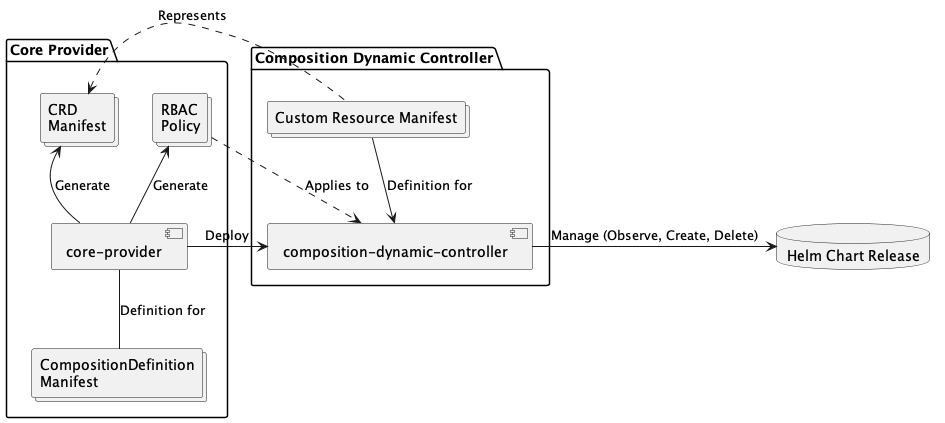
\includegraphics[width=1\linewidth]{images/kraeto_core_provider.png}
    \caption{Krateo Core Provider architecture}
    \label{fig:krateo_core_provider}
\end{figure}

as we can see the core provider deploys the cdc




\section{State of the Art}
An extensive analysis of existing systems have been made in order to...

\subsection{CASPER}

CASPER (Carbon-Aware Scheduling and Provisioning for Distributed Web Services) is a carbon-aware scheduling and provisioning system whose primary purpose is to minimize the carbon footprint of distributed web services \cite{Souza_2023}.
The system is defined as a multi-objective optimization problem that considers two factors: the \textbf{variable carbon intensity} and the \textbf{latency constraints} of the network \cite{Souza_2023}.
By evaluating the framework in real-world scenarios, the authors demonstrate that CASPER achieves significant reductions in carbon emissions (up to 70\%) while meeting application \textbf{Service Level Objectives (SLOs)}, highlighting its potential for practical implementation in large-scale distributed systems \cite{Souza_2023}. However, the system CANNOT BE CONSIDERED A REAL PRODUCTION SYSTEM.




\subsection{CASPIAN}

most important ptobably

\subsection{Let'sWaitAwhile}

test

\subsection{Other systems}

carbonScaler




\subsection{SOTA Recap}

many simulation, no real system
no much flexibility


\newpage
